\documentclass[12pt]{article}
\usepackage{amsmath}
\usepackage{babel}
\usepackage{graphicx}
\usepackage{subcaption}
\usepackage{upgreek}
\usepackage{float}
\usepackage{hyperref}
\usepackage[section]{placeins}
\usepackage{subcaption}
\usepackage{cite}
\usepackage{amssymb}
\usepackage{amsmath}
\usepackage{xepersian}
\settextfont {XB Zar.TTF}
\title{کیهان غیر بی‌دررو و مقایسه‌ی آن با مدل 
$\Lambda CDM$
}
\author{حسین حاتم نیا}
\date{دی 1400}
\begin{document}
\maketitle


\section*{مقدمه}
در کیهان شناسی استاندارد با فرض همگن و همسانگرد و بی دررو بودن کیهان، سعی در توصیف رفتار کیهان در گذشته، حال و آینده داریم. \newline در مدل 
$\Lambda CDM$
 ثابتی در معادلات فریدمان در نظر گرفتیم تا انبساط کیهان که توسط هابل مشاهده شد را توصیف کنیم. اما در ده سال گذشته افرادی سعی در توصیف این انبساط با در نظر گرفتن تغییر آنتروپی در معادله حالت داشتند.
در این حالت کیهان فرایندی غیر بی دررو را طی می‌کند و منبسط می شود. \newline
در این مقاله با در نظر گرفتن جملات اصلاحی در معادلات فریدمان سعی داریم مدلی مناسب برای انبساط کیهان ارائه دهیم و تورم در کیهانی غیر بی دررو
را بررسی کنیم. در نهایت با داده هایی از ابرنواخترها این مدل را با $\Lambda CDM$ مقایسه خواهیم کرد.


\setcounter{section}{-1}
\section{معادله فریدمان و شتاب در کیهان غیر بی دررو}
در معادله ی شتاب به دلیل اثر تغییرات آنتروپی کیهان که همسانگرد هستند، جملاتی اصلاحی به معادله ی شتاب و معادله ی فریدمان اضافه می شود و این آنتروپی با معادله ی زیر داده می شود:
\begin{equation}\label{ent}
S=\frac{k_Bc^3}{G\hbar}\frac{A_H}{4}=\frac{k_Bc^3}{G\hbar}\pi R_H^2=\frac{k_Bc^3}{G\hbar}\pi(\frac{c}{H})^2
\end{equation}
این آنتروپی حاصل اثرات روی سطح افق هابل است. جملات دیگری به این آنتروپی می تواند اضافه شود که بعدا به آن خواهیم پرداخت.\\
معادله ی شتاب با در نظر گرفتن آنتروپی، به صورت کلی به فرم زیر خواهد شد:
\begin{align}
\frac{\ddot a}{a}=H^2+\dot H 
					=-\frac{4\pi G}{3}(\rho + \frac{3P}{c^2})+C_1H^2+C_2\dot H
\end{align}
دلیل این جملات در مقاله [1] آورده شده است.\\
 با در نظر گرفتن معادله حالت هر مولفه 
$P=\omega \rho c^2$
 ، خواهیم داشت:
\begin{equation}
\frac{\ddot a}{a}=-\frac{4\pi G}{3}\rho(1 + 3\omega)+C_1H^2+C_2\dot H
\end{equation}

به همین صورت در معادله فریدمان در کیهان تخت داریم :
\begin{equation}\label{eq:fr}
H^2=(\frac{\dot a}{a})^2=\frac{8\pi G}{3}\rho+C'_1H^2+C'_2 \dot H
\end{equation}
ضرایب موجود در این دو معادله را به روش های تئوری می توان پیدا کرد ولی در اینجا فرم کلی این تصحیح ها را نوشتیم.\\
با ضرب معادله
 \eqref{eq:fr}
 در 
$(1+3\omega)$
 و با استفاده از معادله ی شتاب به سادگی می توان نشان داد:
$$\dot H\propto H^2$$
پس می توان دو جمله اصلاحی در این معادلات را، در یک جمله خلاصه کرد:

\begin{equation}\label{addot}
\frac{\ddot a}{a}=-\frac{4\pi G}{3}(\rho + \frac{3P}{c^2})+CH^2
\end{equation}

\begin{equation}
H^2=(\frac{\dot a}{a})^2=\frac{8\pi G}{3}\rho+C'H^2
\end{equation}
که می توان معادله فریدمان را ساده تر نیز کرد:
\begin{equation}\label{eq:frc}
H^2=(\frac{\dot a}{a})^2=\frac{8\pi G}{3(1-C')}\rho
\end{equation}

با این دو معادله می توانیم همانند مدل استاندارد انبساط کیهان را توصیف کنیم.

در ادامه سعی می کنیم با بررسی مدلی از تغییرات انرژی، انبساط کیهان را بیشتر مورد بررسی قرار دهیم و عبارتی برای عامل مقیاس بر حسب زمان بدست آوریم.
\pagebreak
\section{تصحیح معادله پیوستگی در کیهان غیر بی دررو}
در این بخش تئوری سیستم غیر بی‌دررو را بررسی می کنیم و معادله پیوستگی را با فرض غیر بی‌دررو بودن سیستم بدست می آوریم و سپس با در نظر گرفتن مدل های مختلف 
سعی می کنیم انبساط کیهان را بررسی کنیم.

از قانون اول ترمودینامیک داریم:
\begin{equation}
dE=dQ-dW=dQ-PdV
\end{equation}
با نوشتن انرژی کل بر حسب چگالی انرژی و مشتق گیری از رابطه ی بالا بر حسب زمان خواهیم داشت:

\begin{align}
\dot Q&=\dot E+P\dot V \nonumber \\
		&=\dot\epsilon V+\epsilon\dot V+P\dot V	
\end{align}
 با جایگذاری حجم بر حسب عامل مقیاس خواهیم داشت:
$$V=\frac{4\pi}{3}\chi^3a^3$$
$$\dot V=3\frac{\dot a}{a}V$$

\begin{align}\label{eq:peyvastegi}
\dot Q&=(\dot\epsilon+3\epsilon\frac{\dot a}{a}+3P\frac{\dot a}{a})V \nonumber \\
		&=(\dot\epsilon+3(1+\omega)\epsilon\frac{\dot a}{a})V 
\end{align}
که در  تساوی آخر از معادله ی حالت استفاده کردیم.
 رابطه ی بالا معادله ی پیوستگی در سیستم غیر بی دررو است. اگر $\dot Q=0$ باشد همان معادله پیوستگی در کیهان بی دررو را خواهیم داشت.

\pagebreak
\section{انبساط در کیهان غیر بی دررو}
در این بخش می خواهیم مدلی را بررسی کنیم که انبساط در کیهان را توجیه کند. این انبساط مربوط به کیهان اخیر 
\footnote{
\begin{LTR}
Late Universe
\end{LTR}
}
است و در مورد تورم در کیهان اولیه در بخش بعدی بحث خواهیم کرد.\\
در این مدل فرض می کنیم نرخ انرژی به وجود آمده( یا از بین رفته ) با انرژی داخلی تناسب دارد. 
\begin{equation}
\dot Q=\beta E=\beta\epsilon V
\end{equation}
با استفاده از معادله ی پیوستگی 
\eqref{eq:peyvastegi}
می توان نوشت:
\begin{equation}\label{pey}
\frac{d\epsilon}{\epsilon}+3(1+\omega)\frac{da}{a}-\beta dt=0
\end{equation}
با انتگرال گیری از رابطه ی بالا خواهیم داشت:
\begin{equation}
\epsilon=\epsilon_0a^{-3(1+\omega)}e^{\beta(t-t_0)}
\end{equation}
حال با محاسبه ی عامل مقیاس، سعی در تحلیل انبساط کیهان خواهیم داشت.\\ از معادله ی فریدمان
\eqref{eq:frc}
خواهیم داشت:
\begin{equation}
(\frac{\dot a}{a})^2=\frac{8\pi G\epsilon_0}{3c^2(1-C')}a^{-3(1+\omega)}e^{\beta(t-t_0)}
\end{equation}
با ساده کردن می توان نوشت:
\begin{equation}
\dot a=Ae^{-\frac{1+3\omega}{2}}e^{\frac{\beta t}{2}}
\end{equation}
که در آن A برابر است با:
$$A=\frac{8\pi G\epsilon_0}{3c^2(1-C')}e^{-\beta t_0}$$
با حل این معادله، رابطه ی عامل مقیاس بر حسب زمان برابر خواهد شد با:
\begin{equation}
a(t)=4^{-\frac{1}{3(1+\omega)}}\left( 3(1+\omega)(2Ae^{\frac{\beta t}{2}}\beta^{-1}+\alpha) \right)^{\frac{2}{3(1+\omega)}}
\end{equation}
که در آن $\alpha$ ثابت انتگرال گیری است که باید آن را تعیین کنیم. اگر کیهان آدیاباتیک باشد یعنی $\beta=0$ باشد، در زمان حال $t=t_0$ عامل مقیاس برابر 1 است.
با اعمال کردن این شرایط حدی خواهیم داشت:
$$\alpha=-\frac{2A}{\beta}$$
در نهایت رابطه ی عامل مقیاس با زمان به این صورت داده می شود:
\begin{equation}\label{eq:at}
a(t)=\frac{a(t)}{a(t_0)}=\left(\frac{e^{\beta t/2}-1}{e^{\beta t_0/2}-1}\right)^{\frac{2}{3(1+\omega)}}
\end{equation}
در رابطه ی بالا با میل دادن $\beta$ به سمت صفر خواهیم داشت :
$$a(t)=(t/t_0)^{\frac{2}{3(1+\omega)}}$$
که همان رابطه ای است که انتظار داشتیم.\\
با توجه به رابطه ی عامل مقیاس با زمان
\eqref{eq:at}
، با گذر زمان درصورتی که $\frac{\beta}{(1+\omega)}>0$ باشد، عامل مقیاس افزایش می یابد.

یکی از پارامترهای مهم در کیهان شناسی، پارامتر شتاب است.
\begin{equation}
q=-\frac{\ddot a}{aH^2}
\end{equation}
با محاسبه ی شتاب عامل مقیاس، پارامتر شتاب را می توان به صورت زیر نوشت:
\begin{equation}
q=-1+\frac{3(1+\omega)}{2}e^{-\frac{\beta t}{2}}
\end{equation}
در صورتی که این پارامتر منفی( مثبت ) باشد، انبساط عالم تند شونده( کند شونده ) خواهد بود.
\begin{equation}
q=-1+\frac{3(1+\omega)}{2}e^{-\frac{\beta t}{2}}<0
\end{equation}
\begin{equation}\label{teq}
\implies t_{\ddot a}=-\frac{2\ln{\frac{3}{2}}+\ln(1+\omega)}{\beta}
\end{equation}
با توجه به رابطه ی بالا اگر
 $t>t_{\ddot a}$ 
باشد، کیهان انبساط تند شونده خواهد داشت.\\
در ادامه به پارامتر شتاب باز خواهیم گشت.

\subsection{کیهان ماده غالب غیر بی دررو}
اگر کیهان ماده غالب باشد ($\omega=0$) رابطه ی عامل مقیاس با زمان به این صورت داده می شود:
\begin{equation}\label{eq:a}
a(t)=\left(\frac{e^{\beta t/2}-1}{e^{\beta t_0/2}-1}\right)^{\frac{2}{3}}
\end{equation}

با توجه به رابطه ی 
\eqref{teq}
در صورتی که $\beta$ در این کیهان مثبت باشد مشخص است که در همه‌ی زمان ها، کیهان منبسط می شود و انبساط تند شونده خواهد داشت.
همینطور پارامتر شتاب خواهد شد:
\begin{equation}
q=-1+\frac{3}{2}e^{-\beta t/2}
\end{equation}
با توجه به داده های رصدی از مقاله [5] می توانیم مقدار $q_0$ را در رابطه ی بالا قرار دهیم و خواهیم داشت:
$$q_0\approx -0.4$$

\begin{equation}
\beta t_0=1.833
\end{equation}
حال با رابطه ی عامل مقیاس، می توان پارامتر هابل را محاسبه کرد:
\begin{equation}
H(t)=\frac{\dot a}{a}=\frac{\beta}{3}\frac{1}{1-e^{\beta t/2}}
\end{equation}
با محاسبه ی پارامتر هابل از رابطه ی بالا در زمان حال خواهیم داشت:
\begin{equation}
\frac{\beta}{H_0}=1.800
\end{equation}
حال با حذف $\beta$ در دو رابطه ی بدست آمده بر حسب پارامتر هابل در زمان حال و سن کیهان خواهیم داشت:
$$H_0t_0=\frac{1.833}{1.8}=1.02$$
حال با جایگذاری سن کیهان بر اساس داده های رصدی $t_0=13.8 Gyr$ خواهیم داشت:
\begin{equation}
H_0=72.3\frac{km}{Mpc.s}
\end{equation}
این عدد خیلی به پارامتر هابلی که امروزه از روش های دیگر اندازه گیری شده نزدیک است!

\subsection{انبساط نمایی در کیهان غیر بی دررو}
اگر چگالی انرژی مستقل از زمان و عامل مقیاس باشد($\epsilon=\epsilon_0$) ، پارامتر هابل ثابت خواهد بود($H=H_0$) و در نتیجه عامل مقیاس به صورت نمایی با زمان تغییر می کند که این همان مدل انرژی تاریک است ولی در کیهان 
غیر بی دررو دیگر $\omega=-1$ نخواهد شد. حال سعی می کنیم با حل این مدل، مقداری برای $\omega$ و $\beta$ پیدا کنیم.
می توانیم ثابت هابل 
و معادله ی پیوستگی 
\eqref{pey}
را به این صورت بنویسیم:

\begin{equation}\label{e}
dt=\frac{da}{H_0a}
\end{equation}
\begin{equation}
\frac{d\epsilon_0}{\epsilon_0 da}+\frac{3(1+\omega)}{a}-\beta \frac{dt}{da}=0
\end{equation}
از آنجایی که چگالی انرژی ثابت است، $\frac{d\epsilon_0}{da}=0$ خواهد شد و با جایگذاری $dt$ در معادله ی پیوستگی خواهیم داشت:
\begin{equation}\label{shart}
3(1+\omega)-\beta/H_0=0
\end{equation}
این رابطه، شرطی بین $\omega$ و $\beta$ برقرار می کند که انبساط کیهان به صورت نمایی باشد. 

با حل معادله ی 
\eqref{e}
می توان رابطه ای برای عامل مقیاس به دست آورد.
\begin{equation}
a=a_0e^{H_0(t-t_0)}
\end{equation}
که اگر $ H_0 $ را با توجه به شرطی که در معادله ی 
\eqref{shart}
بدست آوردیم، جایگذاری کنیم، خواهیم داشت:
\begin{equation}
a=a_0e^{\frac{\beta}{3(1+\omega)}(t-t_0)}
\end{equation}
در صورتی که $\frac{\beta}{(1+\omega)}>0$ باشد کیهان انبساط می یابد و در حالتی که $\frac{\beta}{3(1+\omega)}<0$ باشد کیهان با گذر زمان، منقبض می شود.

\pagebreak
\section{تورم}
ما برای پاسخ به یک سری سوالات از جمله تخت بودن کیهان و سطح آخرین پراکندگی، دوره ای را در ابتدای کیهان در نظر گرفتیم که کیهان به صورت نمایی با سرعت زیادی منبسط می شود.
برای پاسخ به این که چه چیزی می تواند این انبساط را توجیه کند، چگالی را ثابت گرفتیم تا عامل مقیاس با زمان به صورت نمایی تغییر کند و فشار مقداری منفی بود که با توجه 
به معادله ی شتاب، شتاب کیهان مقداری مثبت پیدا کند.
در این بخش به این موضوع می پردازیم که در نظر گرفتن آنتروپی، فشار منفی نتیجه می دهد. 

قبلا اثر افق هابل را روی آنتروپی دیدیم و اکنون با در نظر گرفتن اثرات نظریه ریسمان و حالات مختلفی که سیستم می تواند بگیرد که در مقاله [3] آورده شده، رابطه ی آنتروپی 
\eqref{ent}
 خواهد شد:
\begin{align}\label{entc}
S&=\frac{k_Bc^3}{G\hbar}\frac{A_H}{4}+gk_B\ln{\frac{c^3A_H}{G\hbar}}\nonumber \\
 &=\frac{k_BA_H}{4A_p}+gk_B\ln{\frac{A_H}{A_p}}
\end{align}
که در آن $g$ درجه آزادی و مساحت پلانک $A_p$ برابر است با:
$$A_p=\frac{\hbar G}{c^3}$$

نیروی آنتروپیک به صورت زیر تعریف می شود:
\begin{equation}
F=-\frac{dE}{dr}=-T\frac{dS}{dr}
\end{equation}
با مشتق گیری از رابطه ی آنتروپی 
\eqref{entc}
و جایگذاری دمای آنتروپیک
 $T=\frac{\hbar H}{2\pi k_B}$ 
، نیروی آنتروپیک برابر خواهد شد با :
\begin{align}
F&=-\frac{\hbar H}{2\pi k_B}(\frac{k_B}{4A_p}+\frac{gk_BH^2}{\pi c^2})\frac{dA_H}{dr}\nonumber \\
  &=\frac{\hbar H}{2\pi k_B}(\frac{k_Bc^3}{4\hbar G}+\frac{gk_B}{\pi c^2}H^2)(8\pi \frac{c}{H}) \nonumber \\
  &=-\frac{c^4}{G}(1+\frac{4\hbar g}{\pi c^2}H^2)
\end{align}
 فشار حاصل از نیروی آنتروپیک برابر خواهد شد با:
\begin{align}
P&=\frac{F}{A_H}=-\frac{H^2}{4\pi c^2}\frac{c^4}{G}(1+\frac{4\hbar g}{\pi c^2}H^2) \nonumber \\
 &=-\frac{c^2H^2}{4\pi G}(1+\frac{4\hbar g}{\pi c^2}H^2) \nonumber \\
 &=-\frac{2}{3}\epsilon_c (1+\frac{4\hbar g}{\pi c^2}H^2)
\end{align}
که در آن $\epsilon_c$ چگالی انرژی بحرانی است. با توجه به رابطه ی بالا اگر از جمله دوم صرف نظر کنیم و پارامتر چگالی را به این صورت تعریف کنیم:
$$\Omega_i=\frac{\epsilon_i}{\epsilon_c}$$
پارامتر چگالی آنتروپی برابر
 $\frac{2}{3}$ 
خواهد شد که مقداری همیشه ثابت است و خیلی نزدیک به ثابت کیهان شناسی در مدل $\Lambda CDM$ است.\\
با توجه به معادله ی بدست آمده برای فشار، مشخص است که فشار آنتروپیک منفی است و در نتیجه می تواند شتابی مثبتی که در تورم وجود دارد را توجیه کند. می دانیم پارامتر هابل
در کیهان اولیه مقدار خیلی بزرگتری از مقدار امروزی داشته است و در نتیجه این فشار شتاب دهنده به کیهان با گذشت زمان کمتر شده است.

با توجه به معادله ی شتاب
\eqref{addot}
 ، اگر ضریب $H^2$ بزرگتر از جملات قبلی باشد، با حل معادله عامل مقیاس به صورت نمایی با زمان افزایش می یابد و این همان چیزی است 
که در تورم می‌خواهیم تا کیهان سریع متورم شود و شتاب بگیرد.
 در بخش قبلی نیز انبساط نمایی را با این فرض که تغییرات انرژی با خود انرژی متناسب باشد، بررسی کردیم.

با این دو فرض ( فرضی که فشار منفی را بدست آوردیم و همینطور فرض فرم تغییرات انرژی با خود انرژی) می توان عامل مقیاس را به صورت نمایی با زمان زیاد کرد و 
مدلی برای تورم ساخت ولی فرض دوم از تورم خارج نمی شود ولی می توان با در نظر گرفتن فرض اول از تورم خارج شد.
\pagebreak
\section{مقایسه تئوری و داده های رصدی}
می توانیم این مدل ها را با مدل $\Lambda CDM$ با استفاده از داده های موجود از ابرنواختر ها مقایسه کنیم. می خواهیم به
 بهترین منحنی فیت شده به نمودار های مدول فاصله-قرمزگرایی و فاصله درخشندگی-قرمزگرایی نگاه کنیم.
 در این بخش به نمودارهای به دست آمده از داده های ابرنواخترها موجود در مقاله های دیگر نگاهی می اندازیم. \\
با توجه به تعریف فاصله درخشندگی داریم:
\begin{equation}
d_L=\frac{c(1+z)}{H_0}\int_{0}^{z}\frac{dz'}{H(z')}
\end{equation}
که در آن $z$ قرمزگرایی است و با رابطه ی زیر داده می شود:
$$1+z=\frac{a_0}{a}$$
و با توجه به تعریف مدول فاصله ابرنواختر ها داریم:
\begin{equation}
\mu = 5\log{d_L}+25
\end{equation}
که با جایگذاری $H(z')$ مناسب، مدل های مختلف را می توان با داده های ابرنواخترها بررسی کرد.

مدل اولی که می خواهیم بررسی کنیم، کیهان ماده غالبی که قبلا به آن پرداختیم را در نظر می گیریم. نمودار مدول فاصله برحسب قرمزگرایی ابرنواخترهای نوع Ia 
به صورت زیر خواهد شد:
\begin{figure}[H]
\centering
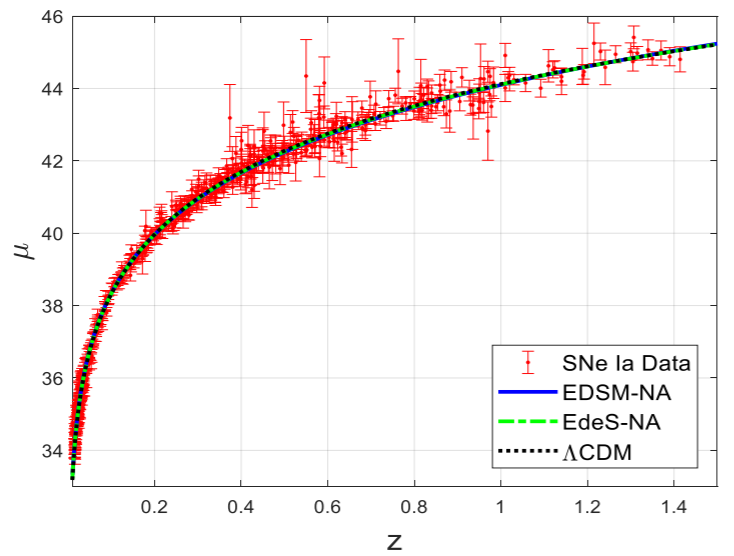
\includegraphics[width=8cm,height=7.5cm]{ax1.png}
\caption*{در این نمودار داده های ابرنواخترها به صورت ارور بار رسم شده اند.
مدل EDSM ، کیهان غیر بی‌دررو ماده غالب با در نظر گرفتن اثر ماخ بر قرمزگرایی ها است و مدل EdeS کیهان غیر بی‌دررو ماده غالب است. مدل $\Lambda CDM$ مدل ماده تاریک سرد و انرژی تاریک که پروسه آدیاباتیک را طی می کند، می باشد.\\
نمودار از مقاله [4] آورده شده است.
}
\end{figure}
همانطور که از نمودارها مشخص است هر دو مدل فیت خوبی برای این داده ها می باشند. اعداد مربوط به دقت منحنی فیت شده در جدول زیر آورده شده.
\begin{figure}[H]
\centering
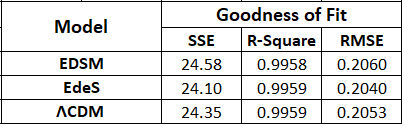
\includegraphics[width=8cm,height=2cm]{ax3.png}
\begin{LTR}
\caption*{
SSE : sum of squares due to errors\\R-Square : coefficient of determination\\RMSE : root mean square error
}
\end{LTR}
\end{figure}
همانطور که از اطلاعات مربوط به خوب فیت شدن منحنی ها مشخص است، مدل کیهان تخت ماده غالب که فرایندی غیر آدیاباتیک را طی می کند، فیت بهتری از 
$\Lambda CDM$ ارائه می دهد.

حال دو مدل دیگر را بررسی می کنیم. همانطور که گفته شد در معادله ی شتاب می توان ضرایب را با فرض های مختلف از تئوری بدست آورد. در اینجا دو مدل را در نظر می گیریم
و نمودار فاصله درخشندگی-قرمزگرایی آن ها را می آوریم.
\begin{equation}\label{mod1}
\frac{\ddot a}{a}=-\frac{4\pi G}{3}(\rho + \frac{3P}{c^2})+H^2
\end{equation}


\begin{equation}\label{mod2}
\frac{\ddot a}{a}=-\frac{4\pi G}{3}(\rho + \frac{3P}{c^2})+\frac{3}{2\pi}H^2+\frac{3}{4\pi}\dot H
\end{equation}

\begin{figure}[H]
\centering
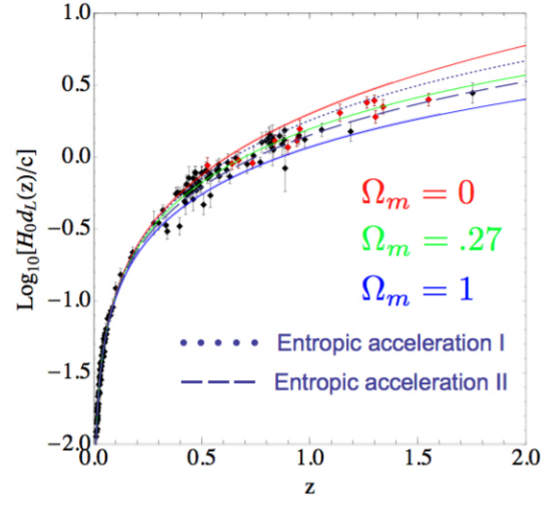
\includegraphics[width=8cm,height=7.5cm]{ax2.png}
\caption*{
مدل 1 با رابطه ی 
\eqref{mod1}
 و مدل 2 با رابطه ی 
\eqref{mod2}
 فیت شده است و با نقطه و دش رسم شده است. مدل $\Lambda CDM$ با $\Omega_m$ های مختلف با خط های پیوسته رسم شده است. این نمودار از مقاله [3] آورده شده است.
}
\end{figure}
این دو مدل نیز فیت خوبی برای این داده ها هستند و نزدیک مدل $\Lambda CDM$ می باشند. 
همانطور که از شکل مشخص است، شتاب دو مدل ارائه شده همانند مدل $\Lambda CDM$ در 
نزدیکی $z=0.5$ تغییر علامت می دهد و شتابی مثبت پیدا می کنند که نکته جالبی است.
\pagebreak
\section{نتیجه گیری}
همانطور که دیدیم با در نظر گرفتن غیر بی دررو بودن کیهان می توانیم انبساط کیهان را توصیف کنیم. با فرض یک مدل ساده برای تغییرات انرژی، ماده غالب بودن کیهان
و با در نظر گرفتن مقدار عددی پارامتر شتاب توانستیم حدود خوبی برای پارامتر هابل در کیهان پیدا کنیم که خیلی نزدیک به پارامتر هابلی است که از داده ها به دست می آیند و حداقل
مانند مدل $\Lambda CDM$ لازم به در نظر گرفتن انرژی تاریک نداشتیم.
سپس توانستیم با در نظر گرفتن آنتروپی کیهان، تورم در جهان اولیه را توصیف کنیم بدون اینکه حضور پتانسیلی برای توجیه این تورم فرض کنیم. در نهایت با مقایسه چند
مدل با داده های رصدی، دقت این مدل ها را بررسی کردیم اما صحت این مدل ها هنوز جای بحث دارد.

\section{منابع}
\begin{latin}
\begin{enumerate}
  \item[[ 1]] \href{https://arxiv.org/pdf/1002.4278.pdf}{Damien A. Easson, Paul H. Frampton, George F. Smoot, Entropic Accelerating Universe(2010)}
  \item[[ 2]] \href{https://arxiv.org/pdf/1208.2482.pdf}{Nobuyoshi Komatsu, Shigeo Kimura, Non-adiabatic-like accelerated expansion of the late universe in entropic cosmology(2013)}
  \item[[ 3]] \href{https://arxiv.org/pdf/1003.1528.pdf}{Damien A. Easson, Paul H. Frampton, George F. Smoot, Entropic Inflation(2012)}
  \item[[ 4]] \href{https://arxiv.org/ftp/arxiv/papers/1810/1810.12090.pdf}{Rajendra P. Gupta, SNe Ia Redshift in a Non-Adiabatic Universe(2018)}
  \item[[ 5]] \href{https://arxiv.org/pdf/1105.1603.pdf}{Ronggen Cai, Zhongliang Tuo, Detecting the cosmic acceleration with current data(2012)}
  \item[[ 6]] \href{https://arxiv.org/pdf/2106.16014.pdf}{Juan Garcia-Bellido, Llorenc Espinosa-Portales, Cosmic acceleration from first principles(2021)}
\end{enumerate}
\end{latin}

\end{document}